\subsection{JTAG* Port}
\label{sec:jtag_port}

The JTAG* port implements a communication link between the \DEBoard~board and its host computer.  
This link can be used by the Quartus\textsuperscript{\textregistered} Prime software to transfer FPGA programming files 
into the \DEBoard~board, and by the \productNameMed{}, discussed in 
Section~\ref{sec:monitor_program}.  The JTAG port also
includes a UART, which can be used to transfer character data between the host computer and
programs that are executing on the \processor~processor.
The programming interface 
of the JTAG UART consists of two 32-bit registers, as shown in Figure \ref{fig:jtag_port}. 
The register mapped to address {\sf 0xFF201000} is called the {\it Data}
register and the register mapped to address {\sf 0xFF201004} is called the {\it Control}
register.

\begin{figure}[h!]
   \begin{center}
       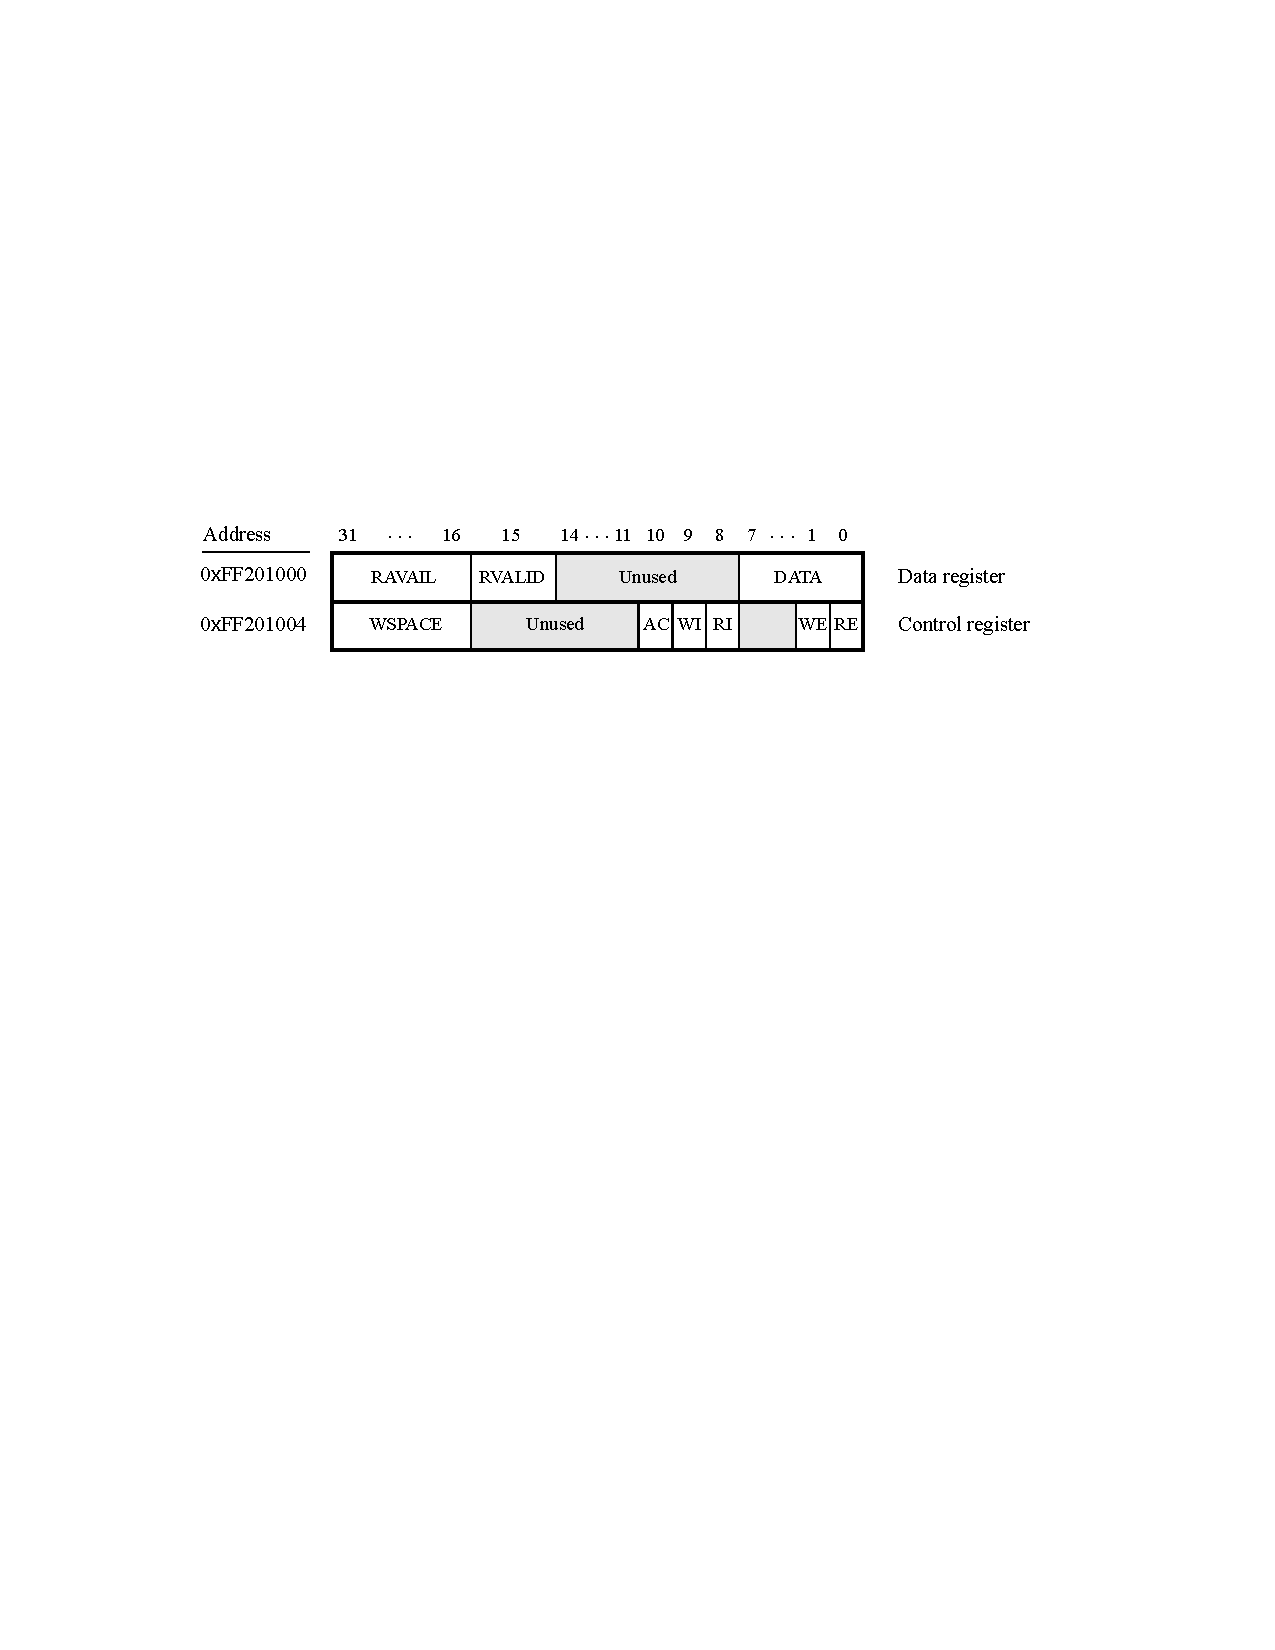
\includegraphics{../../../common/figs/FPGA_JTAG_UART.pdf}
   \end{center}
   \caption{JTAG UART registers.}
	\label{fig:jtag_port}
\end{figure}

When character data from the host computer is received by the JTAG UART 
it is stored in a 64-character FIFO.  The number of characters currently stored in this FIFO is
indicated in the field {\it RAVAIL}, which are
bits 31$-$16 of the {\it Data} register.  If the receive FIFO overflows, then
additional
data is lost. When data is present in the receive FIFO, then the value of {\it RAVAIL} will be 
greater than 0 and the value of bit 15, {\it RVALID}, will be 1. Reading the character at
the head of the FIFO, which is provided in bits $7-0$, decrements the value of {\it RAVAIL} 
by one and returns this decremented value as part of the read
operation. If no data is present in the receive FIFO, then {\it RVALID} will 
be set to 0 and the data in bits $7-0$ is undefined.

The JTAG UART also includes a 64-character FIFO that stores data 
waiting to be transmitted to the host computer. 
Character data is loaded into this FIFO by performing a write to bits 7$-$0
of the {\it Data} register in Figure \ref{fig:jtag_port}.  
Note that writing into this register has no effect 
on received data.  The amount of space, {\it WSPACE}, currently available in the transmit FIFO is 
provided in bits 31$-$16 of the {\it Control} register.  If
the transmit FIFO is full, then any characters written to the {\it Data} register will be lost.

Bit 10 in the {\it Control} register, called {\it AC}, has the value 1 if the JTAG UART has been
accessed by the host computer. This bit can be used to check if a working connection to
the host computer has been established. The {\it AC} bit can be cleared to 0 by writing a 1
into it.

The {\it Control} register bits {\it RE}, {\it WE}, {\it RI}, and {\it WI} are described 
in Section \ref{sec:exceptions}.

\subsubsection{Using the JTAG* UART with Assembly Language Code and C Code}

Listings \ref{lst:jtag_uart_s} and \ref{lst:jtag_uart_C} give simple examples of 
assembly language and C code, respectively, that use the JTAG UART. Both versions of the
code perform the same function, which is to first send an ASCII string to the JTAG UART,
and then enter an endless loop. In the loop, the code reads character data that has 
been received by the JTAG UART, and echoes this data back to the UART for transmission. In
the {\it CPUlator} simulator, there is a JTAG window that allows text to be typed and
echoed. If the program is executed by using the \productNameMed{}, then any keyboard character that 
is typed into the {\it Terminal Window} of the Monitor Program will be 
echoed back, causing the character to appear in the {\it Terminal Window}.

The source code files shown in Listings \ref{lst:jtag_uart_s} and \ref{lst:jtag_uart_C}
are made available as part of the  
\productNameMed{}. The files can be found under the heading {\it sample programs}, 
and are identified by the name {\it JTAG UART}.

